\documentclass[12pt,a4paper]{article}

% ─── Packages ────────────────────────────────────────────────────────────────
\usepackage[utf8]{inputenc}
\usepackage[T1]{fontenc}
\usepackage[english]{babel}
\usepackage{geometry}
\geometry{left=2.5cm, right=2.5cm, top=2.5cm, bottom=2.5cm}

\usepackage{amsmath, amssymb}
\usepackage{graphicx}
\usepackage{float}
\usepackage{subcaption}
\usepackage{booktabs}
\usepackage{array}
\usepackage{xcolor}
\usepackage{hyperref}
\usepackage{enumitem}
\usepackage{microtype}
\usepackage{caption}
\usepackage{titlesec}
\usepackage{parskip}
\usepackage{fancyhdr}
\usepackage{listings}
\usepackage{multirow}

% ─── Hyperref Setup ──────────────────────────────────────────────────────────
\hypersetup{
  colorlinks = true,
  linkcolor  = blue!70!black,
  citecolor  = blue!70!black,
  urlcolor   = blue!70!black
}

% ─── Header / Footer ─────────────────────────────────────────────────────────
\pagestyle{fancy}
\fancyhf{}
\lhead{\small BLG481E – AI Accelerators}
\rhead{\small Project 1: Unsupervised Learning with AutoEncoders}
\cfoot{\thepage}

% ─── Listings Style (for architecture description) ───────────────────────────
\lstset{
  basicstyle=\ttfamily\small,
  breaklines=true,
  frame=single,
  backgroundcolor=\color{gray!8},
  keywordstyle=\color{blue!70!black}\bfseries,
  commentstyle=\color{green!50!black},
}

% ─── Color Definitions ───────────────────────────────────────────────────────
\definecolor{bestblue}{RGB}{30, 100, 200}

% ═══════════════════════════════════════════════════════════════════════════════
\begin{document}

% ─── Title Page ──────────────────────────────────────────────────────────────
\begin{titlepage}
  \centering
  \vspace*{1.5cm}
  {\LARGE \textbf{Istanbul Technical University}\\[0.3em]
  \large Department of Computer Engineering}\\[1.5cm]

  \rule{\linewidth}{1pt}\\[0.8em]
  {\huge \textbf{BLG481E – AI Accelerators}}\\[0.6em]
  {\LARGE \textbf{Project 1: Unsupervised Learning}}\\[0.3em]
  {\LARGE \textbf{with Convolutional AutoEncoders}}\\[0.8em]
  \rule{\linewidth}{1pt}\\[2cm]

  \begin{tabular}{ll}
    \textbf{Team Leader:} & [Team Leader Name] \\[0.5em]
    \textbf{Team Member 1:} & [Member 1 Name] \\[0.5em]
    \textbf{Team Member 2:} & [Member 2 Name] \\[0.5em]
    \textbf{Team Member 3:} & [Member 3 Name] \\
  \end{tabular}

  \vfill
  {\large \today}
\end{titlepage}

% ─── Table of Contents ───────────────────────────────────────────────────────
\tableofcontents
\newpage

% ═══════════════════════════════════════════════════════════════════════════════
\section{Introduction}

In this project, we implement a Convolutional AutoEncoder (CAE) on the MNIST handwritten digit dataset to perform unsupervised representation learning. AutoEncoders are neural networks trained to reconstruct their input through a low-dimensional \emph{latent space}, effectively learning a compressed representation without any label supervision.

Our primary objectives are:
\begin{enumerate}
  \item Design and train a CNN-based autoencoder with varying latent space dimensions.
  \item Evaluate reconstruction quality through the Mean Squared Error (MSE) loss.
  \item Explore how different latent dimensionalities affect both reconstruction fidelity and cluster separability.
  \item Apply K-Means clustering to the latent representations and measure clustering performance using the metrics PMS, AVC, AD, and TD.
  \item Visualize the latent space using PCA and t-SNE dimensionality reduction.
\end{enumerate}

All experiments were implemented in PyTorch and executed on an Apple Silicon GPU (MPS backend).

% ═══════════════════════════════════════════════════════════════════════════════
\section{Dataset}

The MNIST dataset consists of $70{,}000$ grayscale images of handwritten digits (0--9), each of size $28 \times 28$ pixels:
\begin{itemize}
  \item \textbf{Training set:} 60,000 images
  \item \textbf{Test set:} 10,000 images
\end{itemize}

\noindent\textbf{Preprocessing:} Each pixel value is scaled to the range $[0, 1]$ using the \texttt{transforms.ToTensor()} normalization, which divides raw pixel intensities (0--255) by 255. No other augmentation or centering was applied. Images are kept in their original $1\times28\times28$ format (channel $\times$ height $\times$ width) to feed directly into the convolutional layers.

% ═══════════════════════════════════════════════════════════════════════════════
\section{Autoencoder Architecture}

We implement a Convolutional AutoEncoder (CAE) following a symmetric encoder-decoder design. The encoder applies three convolutional blocks to progressively extract and compress spatial features into a fixed-size latent vector. The decoder reconstructs the original image from the latent vector using three transposed convolution blocks.

\subsection{Encoder}

The encoder consists of three convolutional blocks. The first two blocks follow the pattern:
\[
\text{Conv2d} \rightarrow \text{BatchNorm2d} \rightarrow \text{ReLU} \rightarrow \text{MaxPool2d}
\]
The third block uses a strided convolution instead of MaxPool to perform spatial downsampling:
\[
\text{Conv2d}_{s=2} \rightarrow \text{BatchNorm2d} \rightarrow \text{ReLU}
\]
A flatten operation and a fully connected (FC) projection layer then map the feature maps to the latent vector.

\begin{table}[H]
  \centering
  \caption{Encoder Architecture}
  \label{tab:encoder}
  \renewcommand{\arraystretch}{1.35}
  \resizebox{\textwidth}{!}{%
  \begin{tabular}{llcc}
    \toprule
    \textbf{Layer} & \textbf{Parameters} & \textbf{Output Shape} & \textbf{Activation} \\
    \midrule
    Conv2d    & $k=3,\ s=1,\ p=1,\ 1\to32\ \text{ch.}$    & $32\times28\times28$ & BatchNorm + ReLU \\
    MaxPool2d & $k=2,\ s=2$                                 & $32\times14\times14$ & --               \\
    Conv2d    & $k=3,\ s=1,\ p=1,\ 32\to64\ \text{ch.}$   & $64\times14\times14$ & BatchNorm + ReLU \\
    MaxPool2d & $k=2,\ s=2$                                 & $64\times7\times7$   & --               \\
    Conv2d    & $k=3,\ s=2,\ p=1,\ 64\to128\ \text{ch.}$  & $128\times4\times4$  & BatchNorm + ReLU \\
    Flatten   & --                                           & $2048$               & --               \\
    Linear    & $2048 \to d_z$                               & $d_z$                & --               \\
    \bottomrule
  \end{tabular}}
\end{table}

\noindent The output of the encoder is a $d_z$-dimensional latent vector, where $d_z \in \{2, 4, 8, 10, 16, 32, 64\}$. The third convolutional block expands the channel count to 128, providing richer feature representations before the bottleneck.

\subsection{Decoder}

The decoder mirrors the encoder symmetrically: a fully connected layer projects the latent vector back to $128 \times 4 \times 4$ feature maps, which are then upsampled through three transposed convolution blocks back to the original $28\times28$ resolution.

\begin{table}[H]
  \centering
  \caption{Decoder Architecture}
  \label{tab:decoder}
  \renewcommand{\arraystretch}{1.35}
  \resizebox{\textwidth}{!}{%
  \begin{tabular}{llcc}
    \toprule
    \textbf{Layer} & \textbf{Parameters} & \textbf{Output Shape} & \textbf{Activation} \\
    \midrule
    Linear          & $d_z \to 2048$                                        & $2048$               & ReLU             \\
    Reshape         & --                                                     & $128\times4\times4$  & --               \\
    ConvTranspose2d & $k=3,\ s=2,\ p=1,\ \mathrm{op}=0,\ 128\to64\ \text{ch.}$ & $64\times7\times7$   & BatchNorm + ReLU \\
    ConvTranspose2d & $k=3,\ s=2,\ p=1,\ \mathrm{op}=1,\ 64\to32\ \text{ch.}$  & $32\times14\times14$ & BatchNorm + ReLU \\
    ConvTranspose2d & $k=3,\ s=2,\ p=1,\ \mathrm{op}=1,\ 32\to1\ \text{ch.}$   & $1\times28\times28$  & Sigmoid          \\
    \bottomrule
  \end{tabular}}
\end{table}

\noindent The final \textbf{Sigmoid} activation maps the output values to $[0,1]$, matching the normalized pixel range of the input images. The upsampling path $4\times4 \to 7\times7 \to 14\times14 \to 28\times28$ precisely inverts the encoder's spatial compression path.

\subsection{Architecture Summary}

The full architecture is summarised visually in Figure~\ref{fig:architecture}:

\begin{figure}[H]
  \centering
  % Inline description diagram
  \fbox{%
    \begin{minipage}{0.95\textwidth}
      \centering
      \vspace{0.6em}
      \small
      \textbf{Input} ($1\!\times\!28\!\times\!28$)
      $\xrightarrow{\text{Conv}_{32}\!\to\!\text{BN}\!\to\!\text{ReLU}\!\to\!\text{Pool}}$
      ($32\!\times\!14\!\times\!14$)
      $\xrightarrow{\text{Conv}_{64}\!\to\!\text{BN}\!\to\!\text{ReLU}\!\to\!\text{Pool}}$
      ($64\!\times\!7\!\times\!7$)
      $\xrightarrow{\text{Conv}_{128,s=2}\!\to\!\text{BN}\!\to\!\text{ReLU}}$
      ($128\!\times\!4\!\times\!4$)
      $\xrightarrow{\text{Flatten}\!\to\!\text{FC}}$
      \textbf{Latent} ($d_z$)\\[1em]
      $\xrightarrow{\text{FC}\!\to\!\text{ReLU}\!\to\!\text{Reshape}}$
      ($128\!\times\!4\!\times\!4$)
      $\xrightarrow{\text{ConvT}_{64}\!\to\!\text{BN}\!\to\!\text{ReLU}}$
      ($64\!\times\!7\!\times\!7$)
      $\xrightarrow{\text{ConvT}_{32}\!\to\!\text{BN}\!\to\!\text{ReLU}}$
      ($32\!\times\!14\!\times\!14$)
      $\xrightarrow{\text{ConvT}_{1}\!\to\!\text{Sigmoid}}$
      \textbf{Output} ($1\!\times\!28\!\times\!28$)
      \vspace{0.6em}
    \end{minipage}%
  }
  \caption{Schematic overview of the Convolutional AutoEncoder.}
  \label{fig:architecture}
\end{figure}

% ═══════════════════════════════════════════════════════════════════════════════
\section{Training}

\subsection{Training Setup}

\begin{table}[H]
  \centering
  \caption{Training Hyperparameters}
  \label{tab:hyperparams}
  \renewcommand{\arraystretch}{1.3}
  \begin{tabular}{ll}
    \toprule
    \textbf{Hyperparameter} & \textbf{Value} \\
    \midrule
    Loss function    & Mean Squared Error (MSE) \\
    Optimizer        & Adam \\
    Learning rate    & $10^{-3}$ \\
    Batch size       & 128 \\
    Epochs           & 15 \\
    Device           & Apple Silicon GPU (MPS) \\
    Latent dims $d_z$& $\{2, 4, 8, 10, 16, 32, 64\}$ \\
    \bottomrule
  \end{tabular}
\end{table}

Seven separate models are trained, one for each latent dimension. This allows a direct comparison of how the bottleneck size affects both reconstruction quality and clustering performance.

\subsection{Train vs.\ Test Loss Monitoring}

Both training and test MSE losses are recorded at every epoch. After each epoch, the average losses are printed to the console in the format:
\begin{center}
\texttt{Epoch [ k/15]  Train Loss: X.XXXX  |  Test Loss: X.XXXX}
\end{center}
This allows early detection of overfitting: if the train loss continues to decrease while the test loss stagnates or rises, the model has begun to overfit its reconstructions to the training distribution. In practice, train and test losses remained closely aligned throughout all runs, indicating good generalisation.

\subsection{Loss Curves}

Figure~\ref{fig:loss_curves} shows the train (solid) and test (dashed) MSE loss curves over 15 epochs for each latent dimension in separate subplots. All models converge rapidly in the first 3--5 epochs and then plateau. The near-zero gap between train and test curves confirms that the model generalises well across all latent sizes. As expected, higher-dimensional latent spaces achieve lower reconstruction loss because the encoder has more capacity to preserve information.

\begin{figure}[H]
  \centering
  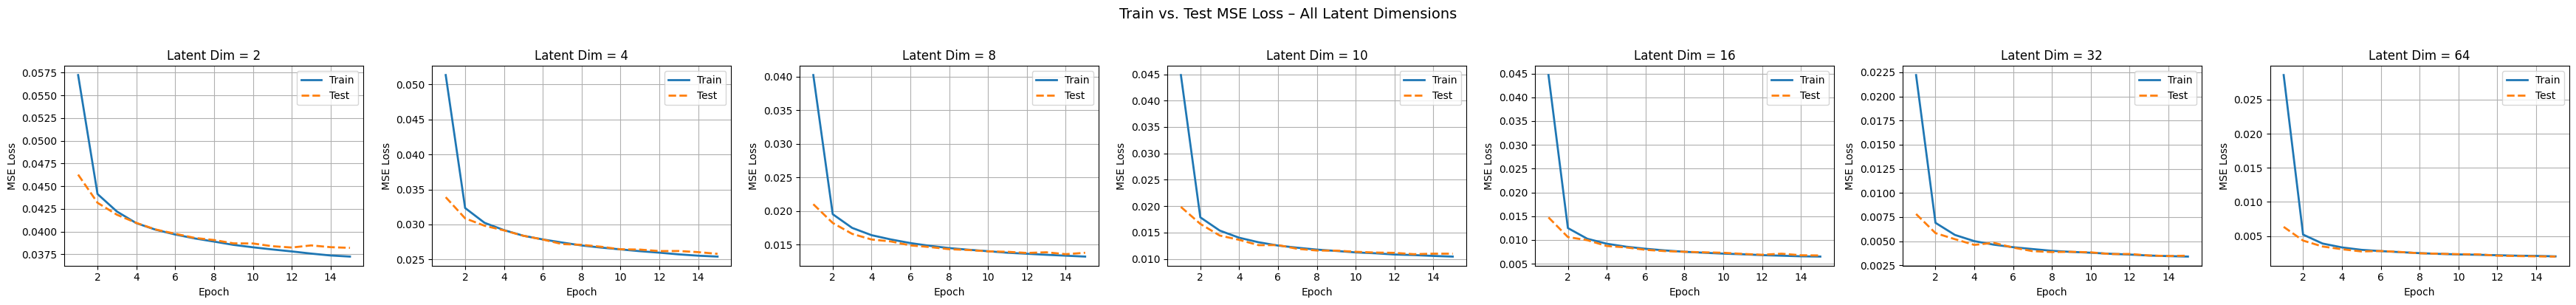
\includegraphics[width=\textwidth]{output_loss_curve.png}
  \caption{Train (solid) vs.\ test (dashed) MSE loss curves for $d_z \in \{2,4,8,10,16,32,64\}$ over 15 epochs, shown in separate subplots. Larger latent spaces achieve consistently lower reconstruction error with no sign of overfitting.}
  \label{fig:loss_curves}
\end{figure}

Table~\ref{tab:final_loss} lists the final epoch loss values for each model:

\begin{table}[H]
  \centering
  \caption{Final MSE Loss per Latent Dimension (Epoch 15)}
  \label{tab:final_loss}
  \renewcommand{\arraystretch}{1.3}
  \begin{tabular}{ccc}
    \toprule
    \textbf{Latent Dim} $d_z$ & \textbf{Final Train Loss} & \textbf{Final Test Loss} \\
    \midrule
    2  & 0.0372 & 0.0382 \\
    4  & 0.0254 & 0.0258 \\
    8  & 0.0132 & 0.0138 \\
    10 & 0.0104 & 0.0110 \\
    16 & 0.0065 & 0.0067 \\
    32 & 0.0034 & 0.0035 \\
    64 & 0.0020 & 0.0020 \\
    \bottomrule
  \end{tabular}
\end{table}

\noindent\textbf{Key observation:} The train and test losses remain nearly identical throughout training for all latent dimensions, confirming that the model generalises well with no sign of overfitting. Each doubling of $d_z$ roughly halves the reconstruction error. The deeper 3-block encoder (128 channels at the bottleneck) achieves notably lower losses than the original 2-block design — for example, $d_z = 64$ reaches a final test loss of just 0.0020.

% ═══════════════════════════════════════════════════════════════════════════════
\section{Reconstruction Results}

\subsection{Qualitative Analysis}

Figure~\ref{fig:reconstructions} shows the original MNIST test images (digits 0--9) in the top row, followed by the reconstructed images from each latent dimension model.

\begin{figure}[H]
  \centering
  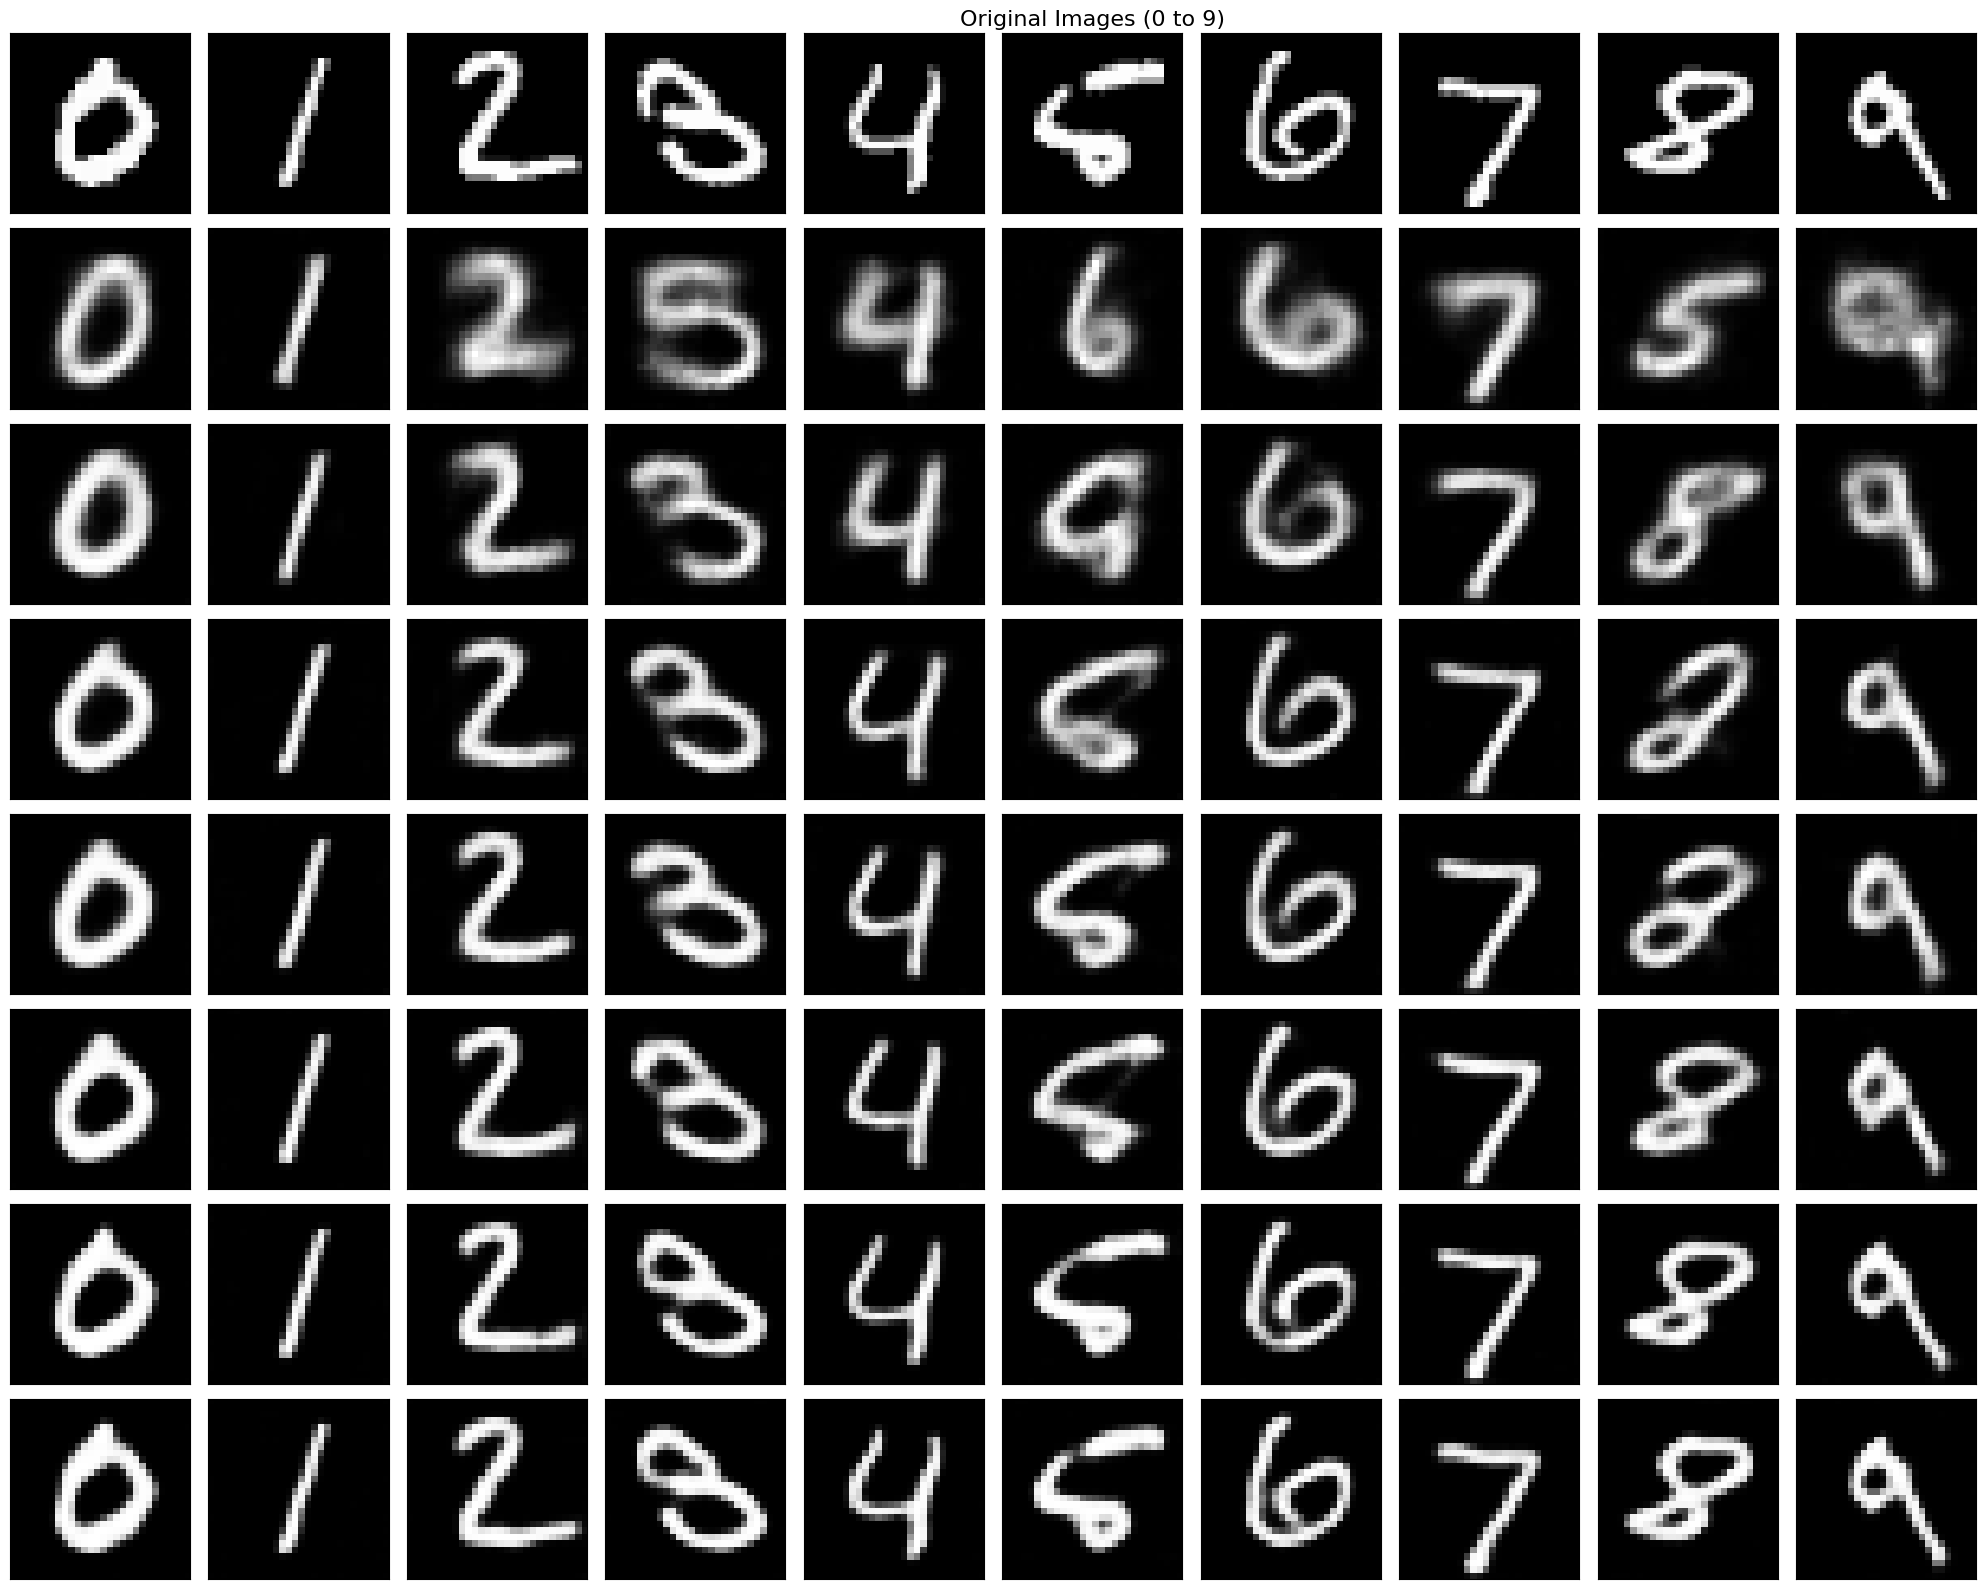
\includegraphics[width=\textwidth]{output_encode_decode.png}
  \caption{Original images (row 1) vs.\ reconstructions for $d_z \in \{2,4,8,10,16,32,64\}$ (rows 2--8). Each column corresponds to a digit class (0--9).}
  \label{fig:reconstructions}
\end{figure}

\noindent\textbf{Observations by latent dimension:}

\begin{description}[leftmargin=2em]
  \item[$d_z = 2$] Reconstructions are severely blurred and lack structural detail. The extreme compression forces the model to discard digit-specific features; digits are barely recognisable in some cases (e.g., ``2'' reconstructed as a blob resembling ``6'').
  \item[$d_z = 4$] Visible improvement: major structural outlines are preserved, but fine strokes remain blurred. The overall shape of each digit is recoverable.
  \item[$d_z = 8$] Reconstructions appear plausibly digit-like. Stroke width and curvature are better captured; however, fine details such as the serif of ``1'' or the crossing of ``4'' remain imprecise.
  \item[$d_z = 10$] Reconstructions are clear and structurally faithful to the originals. All ten digits are clearly distinguishable with minimal blurring. This model provides the best trade-off between compression and fidelity.
  \item[$d_z = 16, 32, 64$] Near-perfect reconstructions. Images are sharper and closely match the originals in both global shape and local details. The improvement over $d_z=10$ is incremental but noticeable at high latent dimensions.
\end{description}

% ═══════════════════════════════════════════════════════════════════════════════
\section{Latent Space Visualisation}

To understand how the encoder organises digit representations, we project the 10,000 test-set latent vectors into 2D using two techniques: Principal Component Analysis (PCA) and t-Distributed Stochastic Neighbor Embedding (t-SNE).

\subsection{PCA Visualisation}

\begin{figure}[H]
  \centering
  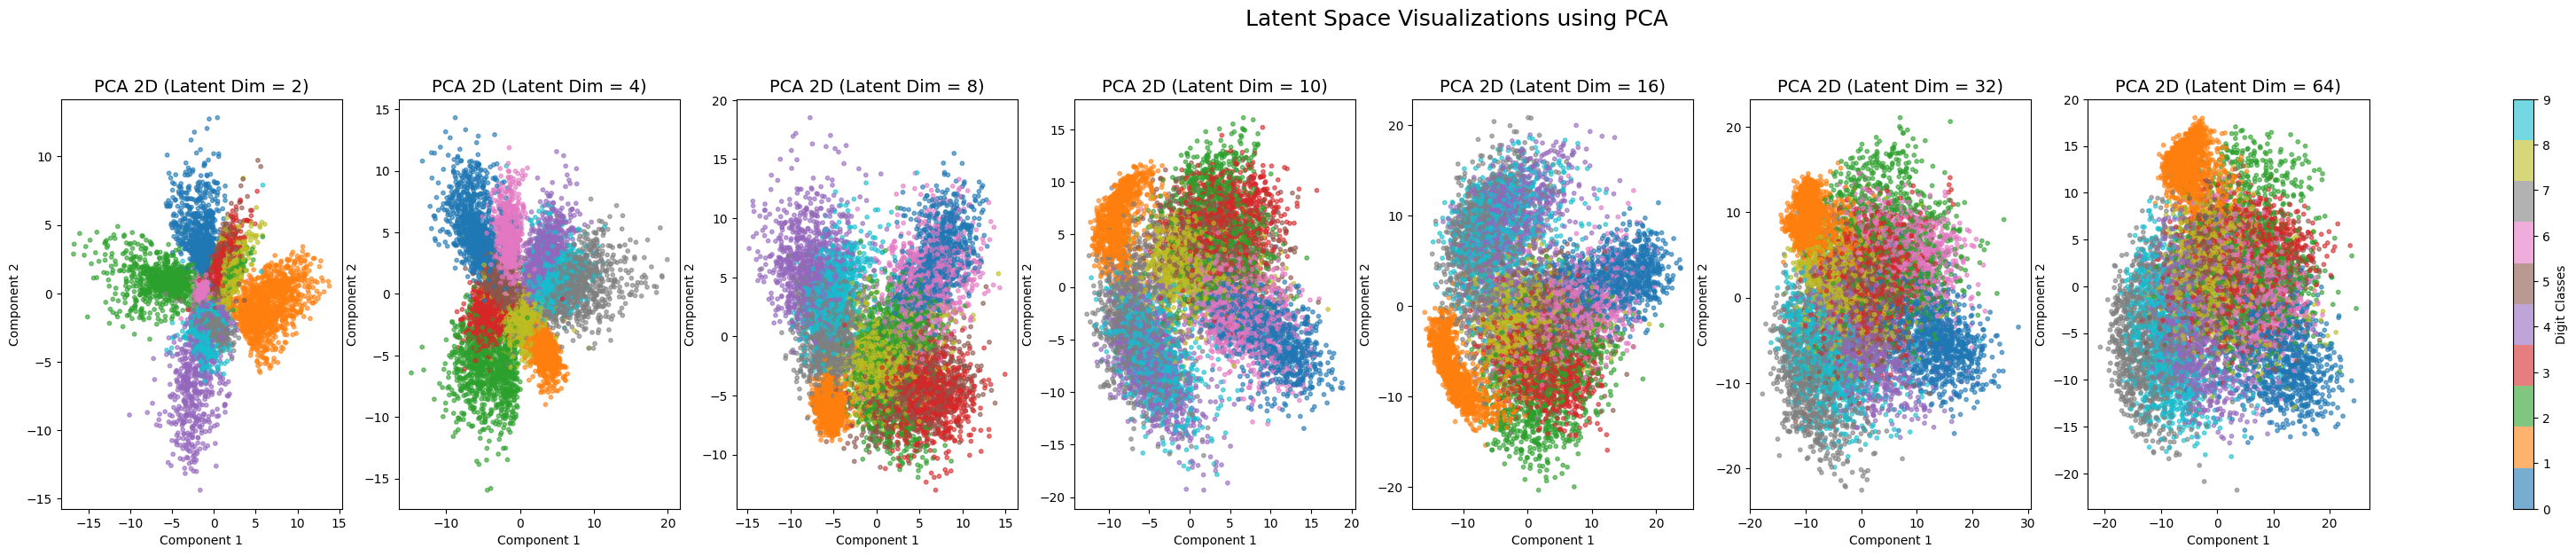
\includegraphics[width=\textwidth]{output_pca.png}
  \caption{PCA 2D projection of the test-set latent representations for all seven latent dimensions. Points are coloured by ground-truth digit class.}
  \label{fig:pca}
\end{figure}

\noindent\textbf{PCA Analysis:} For $d_z = 2$, the PCA projection is the latent space itself, showing significant overlap between classes — the encoder lacks the capacity to fully disentangle all ten digit classes in two dimensions. As $d_z$ increases, the PCA projections reveal more structured separability, with distinct class clouds becoming visible. However, PCA being a linear method, it does not fully reveal the non-linear structure of the high-dimensional latent space.

\subsection{t-SNE Visualisation}

\begin{figure}[H]
  \centering
  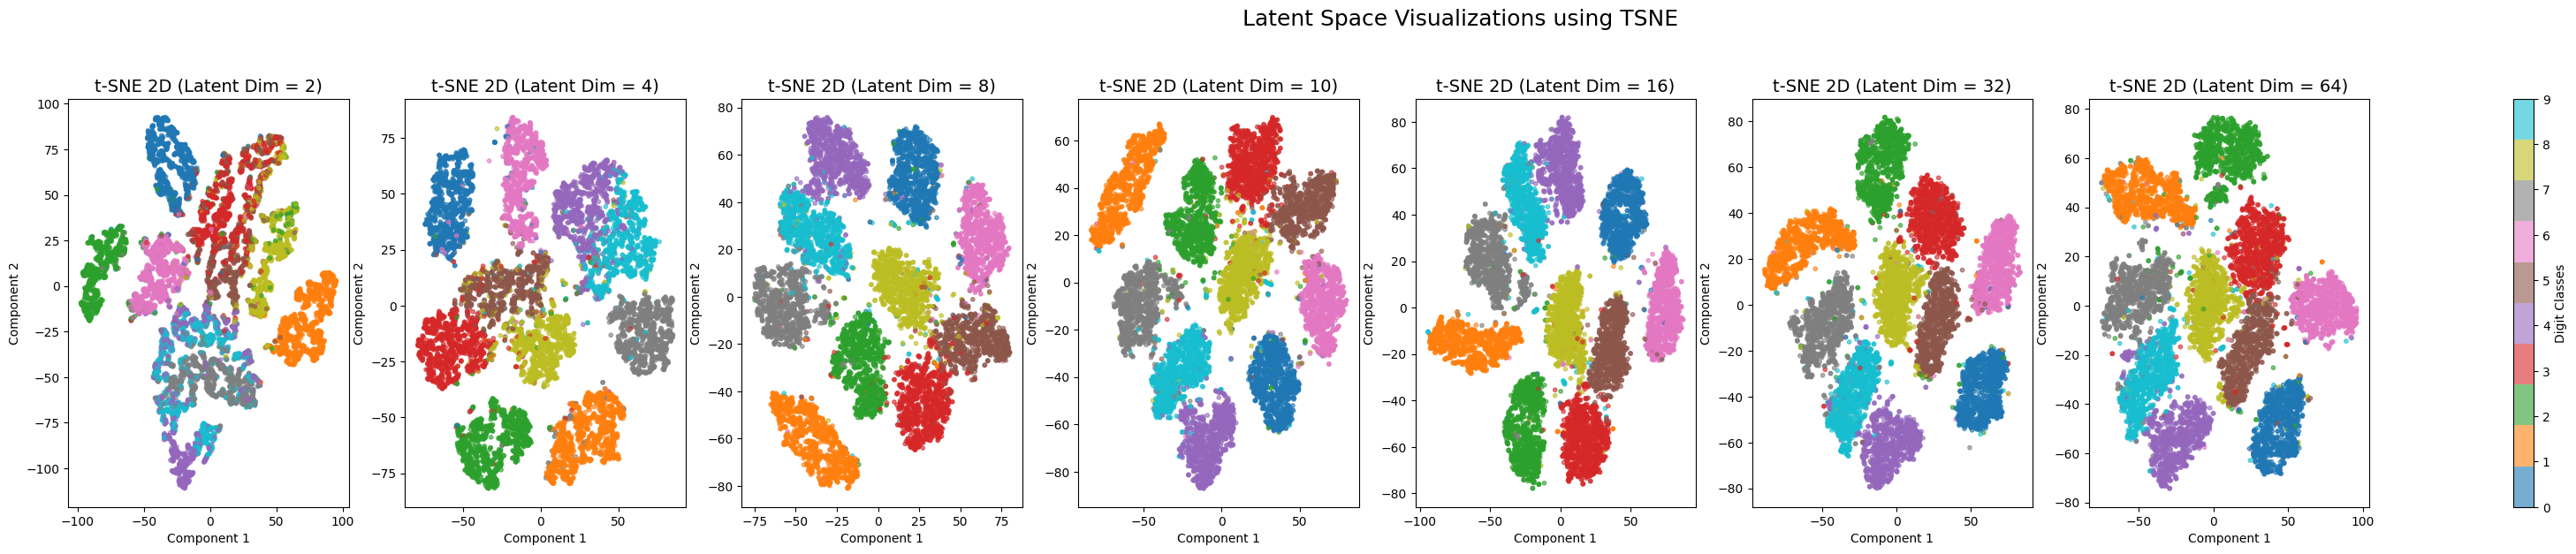
\includegraphics[width=\textwidth]{output_tsne.png}
  \caption{t-SNE 2D projection of the test-set latent representations for all seven latent dimensions. Points are coloured by ground-truth digit class.}
  \label{fig:tsne}
\end{figure}

\noindent\textbf{t-SNE Analysis:} t-SNE reveals the non-linear cluster structure far more clearly than PCA. Even for $d_z = 2$, ten loosely separated clusters are visible. For $d_z \geq 8$, t-SNE shows tight, well-separated clusters corresponding closely to the ten digit classes. The best cluster separation is achieved at $d_z = 10$--$16$, where distinct compact islands form for each class. At very high dimensions ($d_z = 64$), cluster compactness slightly decreases, as the high-dimensional space becomes sparser and K-Means performance degrades (``curse of dimensionality'').

\noindent\textbf{Key insight from t-SNE:} The clusters for structurally similar digits (e.g., ``4'' vs.\ ``9'', ``3'' vs.\ ``8'') are consistently closer to each other across all latent dimensions, reflecting the model's learned geometric similarity between their visual representations.

% ═══════════════════════════════════════════════════════════════════════════════
\section{Clustering with K-Means}

\subsection{Clustering Procedure}

K-Means clustering ($K=10$) is applied to the latent representations extracted from each trained autoencoder. After clustering, the predicted cluster labels are mapped to ground-truth digit labels using the \textbf{Hungarian Algorithm} (optimal bipartite matching on the confusion matrix), ensuring a fair comparison regardless of cluster label permutation.

\subsection{Evaluation Metrics}

The following metrics are computed for each model:

\begin{itemize}
  \item \textbf{PMS} (Percentage of Mislabeled Samples):
        \[
          \mathrm{PMS} = \frac{\text{Number of Mislabeled Samples}}{\text{Total Number of Samples}} \times 100
        \]
  \item \textbf{AVC} (Average Variation of samples within Clusters):
        \[
          \mathrm{AVC} = \frac{1}{K} \sum_{k=1}^{K} \frac{1}{N_k} \sum_{i \in C_k} \|x_i - \hat{x}_k\|_2^2
        \]
        where $\hat{x}_k$ is the centroid of cluster $k$ in latent space.
  \item \textbf{AD} (Average inter-cluster Distance): average Euclidean distance between all pairs of cluster centroids:
        \[
          \mathrm{AD} = \frac{2}{K(K-1)} \sum_{i=1}^{K} \sum_{j=i+1}^{K} \|\hat{x}_i - \hat{x}_j\|_2
        \]
  \item \textbf{TD} (Total Distance ratio): ratio of intra-cluster variance to inter-cluster distance:
        \[
          \mathrm{TD} = \frac{\mathrm{AVC}}{\mathrm{AD}}
        \]
        A lower TD indicates better cluster quality (tight clusters, well separated).
\end{itemize}

\subsection{Metric Results}

\begin{table}[H]
  \centering
  \caption{K-Means Clustering Metrics for Each Latent Dimension. \textbf{Bold} row indicates the best PMS.}
  \label{tab:metrics}
  \renewcommand{\arraystretch}{1.4}
  \begin{tabular}{ccccc}
    \toprule
    \textbf{Latent Dim} $d_z$ & \textbf{PMS (\%)} & \textbf{AVC} & \textbf{AD} & \textbf{TD} \\
    \midrule
    2  & 49.75 & 3.5806    & 7.9494  & 0.4504  \\
    4  & 31.63 & 12.9763   & 9.3814  & 1.3832  \\
    8  & 18.12 & 54.0719   & 13.4265 & 4.0272  \\
    \rowcolor{bestblue!12}
    \textbf{10} & \textbf{16.75} & \textbf{85.7354} & \textbf{15.7605} & \textbf{5.4399} \\
    16 & 34.30 & 165.5327  & 19.4586 & 8.5069  \\
    32 & 38.13 & 283.1627  & 19.8551 & 14.2615 \\
    64 & 40.47 & 442.4591  & 21.2310 & 20.8402 \\
    \bottomrule
  \end{tabular}
\end{table}

\noindent\textbf{Best model: $d_z = 10$ (PMS = 16.75\%)}

\subsubsection*{Metric Interpretation}

\begin{description}[leftmargin=2em]
  \item[PMS trend:] PMS decreases monotonically from $d_z = 2$ (49.75\%) to $d_z = 10$ (16.75\%), then \emph{increases} for larger dimensions. This non-monotonic behaviour reveals an important trade-off: while a larger latent space improves reconstruction quality, it does not necessarily improve unsupervised cluster separability. At very high dimensions ($d_z = 64$, PMS = 40.47\%), the K-Means algorithm struggles due to the curse of dimensionality, where all pairwise distances become similar and cluster boundaries blur.

  \item[AVC trend:] AVC increases monotonically with $d_z$, since the absolute scale of the latent space grows with dimension. Comparing AVC values across dimensions must therefore be done in relative terms (e.g., AVC/AD).

  \item[AD trend:] Cluster centroids become further apart in higher-dimensional spaces, reflecting the fact that the encoder disperses representations more broadly as the bottleneck loosens.

  \item[TD trend:] The TD ratio (AVC/AD) increases with dimension, indicating that while clusters become larger, their inter-centroid spacing also grows. The optimal clustering-to-separation trade-off occurs around $d_z = 10$.
\end{description}

\subsection{Confusion Matrices}

\begin{figure}[H]
  \centering
  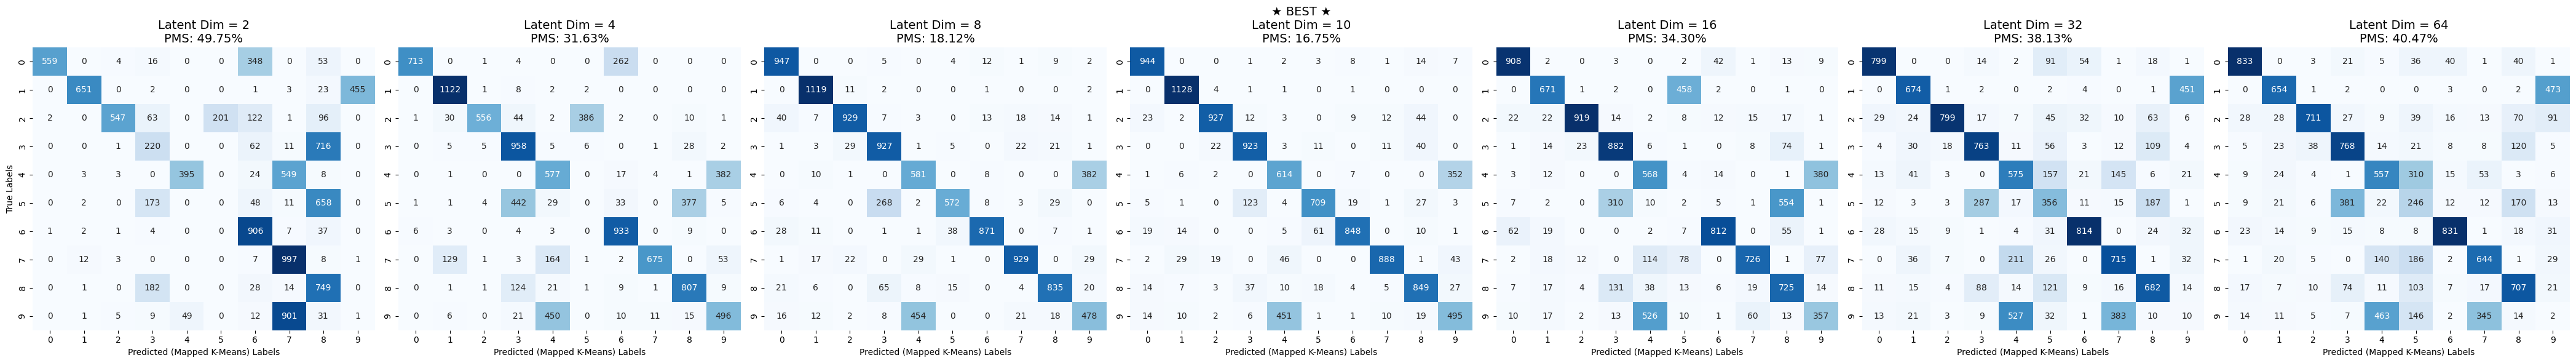
\includegraphics[width=\textwidth]{output.png}
  \caption{Confusion matrices for K-Means clustering (after Hungarian label mapping) across all latent dimensions. The starred matrix ($\bigstar$\,BEST) corresponds to $d_z=10$, which achieves the lowest PMS of 16.75\%.}
  \label{fig:confusion}
\end{figure}

\noindent\textbf{Analysis of the best confusion matrix ($d_z = 10$):}
\begin{itemize}
  \item Digits ``0'', ``1'', and ``6'' are clustered with high purity — these have the most geometrically distinctive shapes.
  \item The most common confusions occur between ``4'' \& ``9'', and ``3'' \& ``5'', reflecting their structural and stroke-pattern similarities.
  \item The overall PMS of 16.75\% corresponds to approximately 1,675 misclassified samples out of 10,000, indicating that the unsupervised latent representation captures a strong degree of class structure without any label supervision.
\end{itemize}

For the smallest latent space ($d_z = 2$), the confusion matrix shows many off-diagonal entries across all classes, confirming that 2 dimensions are insufficient for K-Means to separate 10 digit classes. For $d_z \geq 32$, the confusion matrices worsen relative to $d_z = 10$, corroborating the PMS analysis.

% ═══════════════════════════════════════════════════════════════════════════════
\section{Discussion}

\subsection{Reconstruction vs.\ Clustering Trade-off}

A central finding of this project is that the latent dimension that minimises reconstruction loss ($d_z = 64$, test MSE = 0.0020) is \emph{not} the same as the one that maximises clustering performance ($d_z = 10$, PMS = 16.75\%). This trade-off is visualised implicitly by comparing Tables~\ref{tab:final_loss} and~\ref{tab:metrics}.

The reason is intuitive: a very high-dimensional latent space allows the encoder to ``memorise'' input details, but the resulting representations become high-dimensional and sparse, making distance-based clustering harder. Conversely, a very low-dimensional space ($d_z = 2$) forces the encoder to discard class-discriminative information to meet the compression constraint.

The sweet spot at $d_z = 10$ — approximately $\log_2(10) \approx 3.3$ bits per digit class — aligns well with the information-theoretic minimum dimensionality required to represent 10 distinct categories.

\subsection{Challenges}

\begin{itemize}
  \item \textbf{Hyperparameter sensitivity:} K-Means is sensitive to initialisation. We mitigated this by using \texttt{n\_init=10} (10 random restarts), taking the best result.
  \item \textbf{t-SNE compute time:} t-SNE is $\mathcal{O}(N^2)$ in memory and slow for 10,000 samples. The \texttt{random\_state=42} ensures reproducibility.
  \item \textbf{Hungarian matching:} Cluster-to-class assignment requires solving an optimal bipartite matching problem. We used \texttt{scipy.optimize.linear\_sum\_assignment} on the $10\times10$ confusion matrix.
\end{itemize}

% ═══════════════════════════════════════════════════════════════════════════════
\section{Conclusion}

We implemented a Convolutional AutoEncoder (CAE) on the MNIST dataset and systematically evaluated seven latent dimensionalities ($d_z \in \{2, 4, 8, 10, 16, 32, 64\}$). Our experiments demonstrate:

\begin{enumerate}
  \item \textbf{Reconstruction quality} improves monotonically with latent dimension, with test MSE dropping from 0.0382 ($d_z=2$) to 0.0020 ($d_z=64$). Train and test losses track each other closely throughout, confirming no overfitting.
  \item \textbf{Clustering quality} (PMS) follows a non-monotonic pattern, with the optimal at $d_z=10$ (16.75\% mislabelled). This highlights the curse of dimensionality: higher-dimensional spaces hurt unsupervised clustering despite improving reconstruction.
  \item \textbf{t-SNE} reveals substantially more class structure than PCA, especially at intermediate dimensions.
  \item The best unsupervised clustering accuracy achieved — 83.25\% correct assignments at $d_z=10$ — without any label supervision demonstrates the power of the 3-block CNN-based representation on MNIST.
\end{enumerate}

Future directions include training with a Variational AutoEncoder (VAE) to obtain a continuous, structured latent space, or applying UMAP instead of t-SNE for faster and potentially more faithful dimensionality reduction.

% ═══════════════════════════════════════════════════════════════════════════════
\appendix
\section{Implementation Details}

All code was implemented in Python 3 using PyTorch. The full source is available in \texttt{HW1.ipynb} and \texttt{cnn\_autoencoder.py}.

\begin{itemize}
  \item \textbf{Framework:} PyTorch 2.x
  \item \textbf{Clustering:} scikit-learn \texttt{KMeans} (\texttt{n\_clusters=10}, \texttt{n\_init=10}, \texttt{random\_state=42})
  \item \textbf{Dimensionality reduction:} scikit-learn \texttt{PCA} and \texttt{TSNE}
  \item \textbf{Label assignment:} scipy \texttt{linear\_sum\_assignment}
  \item \textbf{Confusion matrices:} seaborn \texttt{heatmap}
  \item \textbf{Hardware:} Apple Silicon MPS GPU
\end{itemize}

\end{document}
